\documentclass[10pt,twoside,slovak,a4paper]{article}

\usepackage[slovak]{babel}
%\usepackage[T1]{fontenc}
\usepackage[IL2]{fontenc} % lepšia sadzba písmena Ľ než v T1
\usepackage[utf8]{inputenc}
\usepackage{graphicx}
\usepackage{url} % príkaz \url na formátovanie URL
\usepackage{hyperref} % odkazy v texte budú aktívne (pri niektorých triedach dokumentov spôsobuje posun textu)

\usepackage{cite}
%\usepackage{times}

\pagestyle{headings}

\title{Učenie sa cudzích jazykov prostredníctvom mobilu\thanks{Semestrálny projekt v predmete Metódy inžinierskej práce, ak. rok 2020/21, vedenie: Fedor Lehocki}} % meno a priezvisko vyučujúceho na cvičeniach

\author{Marko Stahovec\\[2pt]
	{\small Slovenská technická univerzita v Bratislave}\\
	{\small Fakulta informatiky a informačných technológií}\\
	{\small \texttt{xstahovec@stuba.sk}}
	}

\date{\small 15. október 2020}



\begin{document}

\maketitle

\begin{abstract}
Mobilné zariadenia sa postupom času stali neoddeliteľnou súčasťou našich životov a našej spoločnosti ako celku. Od zariadenia, ktoré slúžilo výlučne na telefonovanie a prenos krátkych textových správ, sa vyvinula pomôcka, vďaka ktorej je náš život mnohonásobne jednoduchší a vďaka ktorej sa dá veľa naučiť. Hlavná charakteristika mobile-learningu je ponímaná ako spôsob výučby, ktorý je spontánny, neformálny a všadeprítomný. Síce takýto spôsob výučby nemusí byť práve najefektívnejší, no učiacemu ponúka široké spektrum možností vrátane slobody, času a predovšetkým priestoru, keďže mobilný telefón je použiteľný takmer v akejkoľvek situácii. A preto sa v tejto práci budeme venovať kladom a záporom, t.j. ľahkej dostupnosti, individuálnosti, ale aj nevýhodám malej obrazovky, ukladaniu dát apod. Taktiež sa dotkneme spôsobov, akými by sa dalo také učenie realizovať a taktiež schopnostiam, ktoré sa daným štýlom učenia môžu bohato rozvíjať, napr. gramatika, porozumenie, slovná zásoba apod.
\end{abstract}



\section{Úvod}


Vo svete, v ktorom sa technické zariadenia veľmi rýchlo rozvíjajú, sa bezdrôtová komunikačná technológia nachádza niekde na čele už nezastaviteľného pokroku\cite{Miangah2012}. Každým dňom sa jej pokrytie dostáva hlbšie a hlbľšie do našich životov a učenie sa nie je nijakou výnimkou. Ukázalo sa, že použitie týchto technológií na edukačné účely je v súlade so strategickými vzdelávacími cieľmi, ako je zlepšenie pozornosti a prospechu študentov, podpora diferenciácie učebných potrieb a v neposlednom rade aj oslovovanie študentov, ktorí by inak nemali príležitosť zúčastňovať sa na vzdelávaní\cite{KukulskaHulme2009}. Veľké úsilie sa venovalo aj pochopeniu toho, ako mobilné technológie súvisia s tradičnými aj inovatívnymi spôsobmi výučby a učenia, ukazovaniu použiteľnosti mobilného učenia v širokom spektre aktivít a zdôrazňovaniu najdôležitejších vynárajúcich sa problémov\cite{KukulskaHulme2009}. 

S príchodom internetu všetky možnosti a uplatnenia takéhoto štýlu učenia začali vzrastať exponenciálne, keďže od jednoduchých pracovných listov a učebníc dostupných na internete sa prešlo k praktickým spôsobom, ako je napríklad ponuka audio knihy pri bookovaní dovolenky, ktorá pozostáva z bežnej slovnej zásoby v danom cudzom jazyku podľa danej krajiny. Vzhľadom na mobilné zariadenia konkrétne, tie už do istej miery vďaka svojej všadeprítomnosti ovplyvňujú to, ako sa ľudia učia; na druhej strane je potrebné, aby pedagógovia túto skutočnosť využívali vo svoj prospech\cite{KukulskaHulme2009}. Výhody práve týchto zariadení sú efektívne uplatňované na vedných predmetoch ako sú geografia a biológia, kde sa obsah učiva dá jednoducho graficky spracovať, no podobný prístup sa dá uplatniť aj na cudzie jazyky.

Cieľom tohto článku je zamyslieť sa nad tým, čo mobile-learning ponúka, a znázorniť, v čom tento spôsob výučby vyniká a kde naopak zaostáva. Zameriame sa na výučbu jazykových schopností prostredníctvom mobilného zariadenia (mobile assisted language learning - ďalej len \emph{MALL}), uvedieme schopnosti, ktoré sa takto primárne rozvíjajú, kriticky zohľadníme výhody a nevýhody tohto princípu a na záver sa pozrieme aj na jeden konkrétny experimentálny príklad z praxe. No predtým, ako sa pozrieme na konkrétne príklady, je dôležité si objasniť, čo sa rozumie pod pojmom "mobile learning".


\section{Mobile learning} \label{ml}

Vysoká popularita mobilných zariadení má za následok okrem zmeny našich životných štýlov aj trendy v učení a komunikácii. No aj napriek tejto všadeprítomnej prezencie zatiaľ neexistuje jednoznačná definícia pre "mobile learning"\cite{Kim2012}. Čiastočne je to preto, lebo táto oblasť podlieha rapídnej evolúcii, a čiastočne pre nejednoznačnosť pojmu "mobile", ktorý môže mať viacero významov. Mobilitu je potrebné chápať nielen z hľadiska priestorového pohybu, ale aj spôsobov, ako môže tento pohyb umožniť posúvanie času a prekračovanie hraníc\cite{KukulskaHulme2009}. Netreba zabúdať na fakt, že technologický progres je ako loď na otvorenom mori, a tak nemožno jasne predpokladať, či používanie mobilného telefónu bude rozšírené v takej podobe, ako je tomu dnes. 

Na druhej strane je možné tvrdiť, že zariadenia, ktoré študenti používajú, nie sú relevantné; dôležitá je predstava mobility a budovanie učebných postupov v tomto procese\cite{KukulskaHulme2009}. El-Hussein a Cronje (2010) definovali koncept mobility v troch oblastiach: mobilita technológie, mobilita učenia a mobilita študenta\cite{Kim2012}. 

Mobilitu technológie možno zhrnúť do niekoľkých pojmov, t.j. smartfóny, digitálne kamery, notebooky, GPS zariadenia alebo iné technológie, ktoré sú vybavené bezdrôtovým aplikačným protokolom. Takéto mobilné technológie umožňujú používateľom vykonávať rôzne sociálno-interaktívne činnosti vrátane komunikácie, používania aplikácií, zberu informácií či relaxu\cite{Kim2012}.

Mobilitu učenia definuje niekoľko prívlastkov, ktoré charakterizujú nové možnosti edukačného prístupu: personalizovaný, zameraný na študenta, situovaný, spolupracujúci a všadeprítomný. Študenti majú v takýchto podmienkach osobné a jedinečné skúsenosti v kontexte, v ktorom sa nachádzajú. Pokiaľ ide o vek, miesto, čas alebo trvanie, tak tie nepredstavujú nijaké obmedzenia\cite{Kim2012}. 

A v neposlednom rade kladie mobile learning dôraz na individualitu študentov, ktorým sa podmienky prisposôbujú podľa ich vlastných potrieb. Práve vďaka tomu môže byť ich študijný progres čo najefektívnejší a najproduktívnejší.

%Z obr.~\ref{f:rozhod} je všetko jasné. 
%\begin{figure*}[tbh]
%\centering
%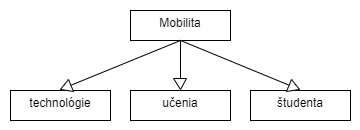
\includegraphics[scale=1.0]{diagram.pdf}
%\caption{Rozhodujúci argument.}
%\label{f:rozhod}
%\end{figure*}


\section{MALL a schopnosti, ktoré obohacuje} \label{mall}

Základným problémom je teda\ldots{} Najprv sa pozrieme na nejaké vysvetlenie (časť~\ref{ina:nejake}), a potom na ešte nejaké (časť~\ref{ina:nejake}).\footnote{Niekedy môžete potrebovať aj poznámku pod čiarou.}

Môže sa zdať, že problém vlastne nejestvuje\cite{Miangah2012}, ale bolo dokázané, že to tak nie je~\cite{KukulskaHulme2009}. Napriek tomu\, aj dnes na webe narazíme na všelijaké pochybné názory\cite{Kim2012}. Dôležité veci\cite{Azar2014} možno \emph{zdôrazniť kurzívou}.


\subsection{Slovná zásoba} \label{mall:slovnazasoba}

Niekedy treba uviesť zoznam:

\begin{enumerate}
\item jedna vec
\item druhá vec
	\begin{enumerate}
	\item x
	\item y
	\end{enumerate}
\end{enumerate}


\subsection{Porozumenie} \label{mall:porozumenie}

\paragraph{Chápanie textu.}
Niekedy je potrebné nadpisom označiť odsek. Text pokračuje hneď za nadpisom.



\section{Výhody a nevýhody} \label{vyhodyanevyhody}

Je potrebný aj obrázok/graf/tabuľka.



\section{Experiment} \label{experiment}




\section{Záver} \label{zaver} % prípadne iný variant názvu



%\acknowledgement{Ak niekomu chcete poďakovať}


% týmto sa generuje zoznam literatúry z obsahu súboru literatura.bib
\bibliography{literatura}
\bibliographystyle{plain} % prípadne alpha, abbrv alebo hociktorý iný
\end{document}
